% !TeX program = xelatex
% Japanese mathematical working note; all diagrams are native TikZ.
\documentclass[11pt,a4paper]{article}
\usepackage[margin=22mm,top=23mm,bottom=23mm]{geometry}
\usepackage{fontspec}
\usepackage{xeCJK}
\setmainfont{Liberation Serif}
\setsansfont{Liberation Sans}
\setmonofont{DejaVu Sans Mono}[Scale=0.87]
\setCJKmainfont{Noto Serif CJK JP}
\setCJKsansfont{Noto Sans CJK JP}
\setCJKmonofont{Noto Sans Mono CJK JP}
\usepackage{amsmath,amssymb,amsthm,mathtools}
\usepackage{microtype}
\usepackage{booktabs,array,tabularx,multirow,longtable}
\usepackage{tikz}
\usetikzlibrary{arrows.meta,calc,angles,quotes,decorations.pathreplacing,patterns,positioning,backgrounds,fit,shapes.geometric}
\usepackage[most]{tcolorbox}
\usepackage{enumitem}
\usepackage{caption}
\usepackage{fancyhdr}
\usepackage{hyperref}
\usepackage{cleveref}
\usepackage{xcolor}
\usepackage{float}
\usepackage{needspace}
\hypersetup{colorlinks=true,linkcolor=blue!55!black,urlcolor=blue!55!black,citecolor=blue!55!black,pdftitle={15等円の最小外接円パッキング：厳密補題と未解決の大域排除},pdfauthor={Research working note}}
\definecolor{ink}{HTML}{17304E}
\definecolor{sea}{HTML}{357D9B}
\definecolor{amber}{HTML}{B97C32}
\definecolor{mint}{HTML}{407B64}
\definecolor{faint}{HTML}{F1F5F8}
\definecolor{alert}{HTML}{993F43}
\renewcommand{\arraystretch}{1.22}
\setlength{\parindent}{1em}
\setlength{\parskip}{3pt}
\setlist[itemize]{itemsep=2pt,topsep=5pt,leftmargin=2em}
\setlist[enumerate]{itemsep=3pt,topsep=5pt,leftmargin=2.3em}
\newtheoremstyle{JPthm}{7pt}{7pt}{\normalfont}{}{\bfseries\color{ink}}{.}{.6em}{}
\theoremstyle{JPthm}
\newtheorem{theorem}{定理}[section]
\newtheorem{lemma}[theorem]{補題}
\newtheorem{proposition}[theorem]{命題}
\newtheorem{corollary}[theorem]{系}
\newtheorem{observation}[theorem]{観察}
\theoremstyle{definition}
\newtheorem{definition}[theorem]{定義}
\newtheorem{problem}[theorem]{未解決課題}
\renewcommand{\proofname}{証明}
\newcommand{\Rstar}{R_{15}^{*}}
\newcommand{\Rc}{R_{0}}
\newcommand{\ph}{\varphi}
\newcommand{\angles}{\operatorname{ang}}
\newcommand{\one}{\mathbf 1}
\newtcolorbox{statusbox}[1][]{colback=faint,colframe=sea!50!black,boxrule=.65pt,arc=2pt,top=7pt,bottom=7pt,left=10pt,right=10pt,#1}
\newtcolorbox{warningbox}[1][]{colback=red!2,colframe=alert!55,boxrule=.8pt,arc=2pt,top=8pt,bottom=8pt,left=10pt,right=10pt,#1}
\newtcolorbox{keybox}[1][]{colback=white,colframe=ink!65,boxrule=1.0pt,arc=2pt,top=8pt,bottom=8pt,left=10pt,right=10pt,#1}
\captionsetup{font=small,labelfont={bf,color=ink},skip=5pt}
\pagestyle{fancy}
\fancyhf{}
\fancyhead[L]{\sffamily\small 15等円の最小外接円パッキング}
\fancyhead[R]{\sffamily\small Working note · 2026-10-09}
\fancyfoot[C]{\thepage}
\renewcommand{\headrulewidth}{0.3pt}
\setlength{\headheight}{15pt}
\tikzset{unitdisk/.style={draw=ink!72,fill=sea!22,line width=.5pt}, innerdisk/.style={draw=ink!70,fill=amber!44,line width=.55pt},outerdisk/.style={draw=ink!72,fill=sea!25,line width=.55pt},geoline/.style={line width=.85pt,ink},guideline/.style={line width=.65pt,ink!55,densely dashed}, note/.style={font=\footnotesize\sffamily,align=center},alertline/.style={draw=alert,very thick},nodebubble/.style={draw=ink,rounded corners=2pt,fill=white,inner sep=5pt,font=\footnotesize\sffamily,align=center}}
\begin{document}
\begin{center}
{\sffamily\color{ink}\LARGE\bfseries 15等円の最小外接円パッキング}\par
\vspace{3mm}
{\sffamily\large 候補配置・厳密な幾何学的削減・角度障壁・証明書設計}\par
\vspace{3mm}
{\color{sea}\rule{.76\linewidth}{1pt}}\par
\vspace{2mm}
{\small 研究ノート（証明の途中経過）\quad | \quad 2026年10月9日}
\end{center}
\vspace{3mm}
\begin{warningbox}
\textbf{重要：15等円の大域最適性は本稿では証明されていない。}\quad
本稿は、厳密に証明できる候補配置の上界、内外の個数制限、巡回分類、局所角度障壁と、未解決の大域排除問題をまとめた研究ノートである。
計算機による負閉路の例は探索上の証拠であって、全配置の証明書ではない。
\end{warningbox}
\begin{abstract}
半径1の合同な円15個を、重なりなく収容する最小の円形容器の半径を $\Rstar$ とする。
既知の $D_5$ 対称候補から、
$\Rc=1+\sqrt{1+(2+\cot(\pi/5))^2}=4.5213569647\ldots$
という厳密な上界を得る。
中心距離 $s$ のしきい値 $L=(\Rc-1)-4/(\Rc-1)$ により、
任意の候補配置では内側の中心数が5--8、外側が7--10であることを示す。
合同円の交換対称性を利用すると、内外の巡回パターンは二面体群同値で760種類となる。
さらに候補配置近傍の $(I,O,O)^5$ 型を、5変数の角度障壁で排除する。
全760クラスにおける連続的な中心距離の大域排除は残された課題である。
\end{abstract}
\tableofcontents
\clearpage

\section{問題設定と現在の到達点}
半径1の閉円板 $D_i=\overline B(p_i,1)\subset\mathbb R^2$ が互いに内部を共有せず、
中心を原点とする半径 $R$ の閉円板に収納される条件は、
\begin{align}
\lVert p_i\rVert &\le R-1 \quad (1\le i\le15),\label{eq:wall}\\
\lVert p_i-p_j\rVert&\ge2\quad(1\le i<j\le15).\label{eq:pair}
\end{align}
最小の $R$ を $\Rstar$ と書く。中心が原点に一致する場合も含める。

\begin{statusbox}
\textbf{本稿の結論の階層}\par
\textcolor{mint}{\textbf{証明済み：}} $\Rstar\le\Rc$、内外5--8分類、760個の巡回パターン、固定半径での角度差制約、候補近傍の局所排除。\par
\textcolor{amber}{\textbf{数値実験：}} 一部の非対称な半径ベクトルに対し負閉路を検出。\par
\textcolor{alert}{\textbf{未証明：}} $\Rstar\ge\Rc$。そのため $\Rstar=\Rc$ は現時点では\textbf{予想}である。
\end{statusbox}

\subsection{先行研究における位置づけ}
Packomaniaの合同円パッキング表には、15等円の最良既知の半径として
$4.521356964706164\ldots$ が掲載されている\cite{packomania}。\par
2024年のEkanayake--LaFountainによる14等円の最適性証明は、
とくに有用な比較対象である\cite{ekanayake}。
同じ円形容器問題でも、特定の対称配置を\emph{構成}することと、すべての非対称配置を排除して\emph{大域最適性を証明}することは別である。

\section{既知の15円配置を厳密に構成する}
\subsection{中心座標と候補半径}
\begin{definition}[候補半径と接触配置]\label{def:candidate}
\begin{gather}
\phi=\frac\pi5,\qquad a=\csc\phi,\qquad
b=\sqrt{1+(2+\cot\phi)^2},\\
\alpha=\phi-\arcsin(1/b),\qquad \Rc=1+b.
\end{gather}
$k=0,\ldots,4$ に対し、中心を極座標で
\begin{equation}\label{eq:center-coords}
I_k=(a,2k\phi),\qquad O_k^-=(b,2k\phi-\alpha),\qquad
O_k^+=(b,2k\phi+\alpha)
\end{equation}
と定め、各中心のまわりに半径1の円板を置く。
\end{definition}

\begin{figure}[H]
\centering
\begin{tikzpicture}[scale=.8]
\pgfmathsetmacro{\ar}{1/sin(36)}
\pgfmathsetmacro{\br}{sqrt(1+(2+1/tan(36))^2)}
\pgfmathsetmacro{\RR}{1+\br}
\pgfmathsetmacro{\al}{36-asin(1/\br)}
\draw[fill=sea!3,draw=ink,line width=1.25pt] (0,0) circle[radius=\RR];
\draw[guideline] (0,0) circle[radius=\br];
\draw[guideline] (0,0) circle[radius=\ar];
\foreach \k in {0,1,...,4} {
 \pgfmathsetmacro{\t}{72*\k+90}
 \draw[innerdisk] (\t:\ar) circle[radius=1];
 \draw[outerdisk] (\t-\al:\br) circle[radius=1];
 \draw[outerdisk] (\t+\al:\br) circle[radius=1];
 \fill[ink] (\t:\ar) circle[radius=.034];
}
\draw[guideline] (0,0)--(90:\ar);
\draw[guideline] (0,0)--({90-\al}:\br);
\draw[<->,line width=.75pt,sea] (155:\br+.20) arc[start angle=155,end angle=228,radius=\br+.20];
\node[note,fill=white,inner sep=2pt] at (0,-.17) {$O$};
\node[note,anchor=west] at (4.9,3.45) {外側10円は壁に接触};
\draw[sea,-{Latex[length=2mm]}] (4.85,3.17)--(3.3,2.65);
\node[note,anchor=west] at (4.85,-3.0) {内側5円が正五角形};
\draw[amber,-{Latex[length=2mm]}] (4.85,-2.75)--(1.4,-1.5);
\node[note,anchor=west] at (4.85,.2) {$R_0=1+b$};
\end{tikzpicture}
\caption{15等円の既知 $D_5$ 対称候補（定義\ref{def:candidate}の厳密座標によるTikZ作図）。図中の円は単位円、破線は円中心の補助円。}
\label{fig:candidate}
\end{figure}

\begin{lemma}[候補配置は重ならない]\label{lem:construct}
定義\ref{def:candidate}の15円板は互いに内部が重ならず、半径 $\Rc$ の容器内に収まる。
したがって $\Rstar\le\Rc$ である。
\end{lemma}
\begin{proof}
内側の隣接中心間距離は $2a\sin\phi=2$。
外側の中心角は交互に $2\alpha$ と $2(\phi-\alpha)$ であり、
後者について
\[
2b\sin(\phi-\alpha)=2
\]
が成り立つ。$2\alpha>2(\phi-\alpha)$ なので、外側の隣接円同士は重ならない。
内側・外側について、$a\sin\phi=1$ と
$\sqrt{b^2-1}=2+\cot\phi$ を使うと
\[
 a^2+b^2-2ab\cos\alpha=4
\]
を得る。内外の中心角の絶対値の最小値は $\alpha$ であるから、その他の内外ペアも距離が2以上。
同じ半径の中心同士は角度差の小さいペアが距離を最小にするので、非隣接ペアも問題ない。
容器条件について、外側中心距離は $b=\Rc-1$、内側は $a<b$ である。よって成立する。
\end{proof}

\begin{figure}[H]
\centering
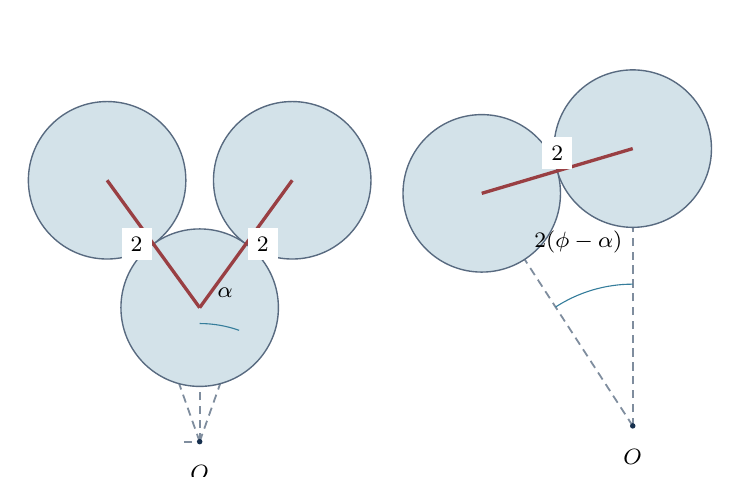
\begin{tikzpicture}[scale=1.0]
\pgfmathsetmacro{\aa}{1/sin(36)} \pgfmathsetmacro{\bb}{sqrt(1+(2+1/tan(36))^2)} \pgfmathsetmacro{\al}{36-asin(1/\bb)}
\coordinate (O) at (0,0);
\coordinate (I) at (90:\aa); \coordinate (M) at ({90-\al}:\bb);\coordinate (P) at ({90+\al}:\bb);
\draw[guideline] (-.2,0)--(O);
\draw[guideline] (O)--(I) node[midway,left,note] {$a$};
\draw[guideline] (O)--(M) node[midway,right,note] {$b$};
\draw[guideline] (O)--(P);
\draw[unitdisk] (I) circle[radius=1];
\draw[unitdisk] (M) circle[radius=1];
\draw[unitdisk] (P) circle[radius=1];
\draw[alertline] (I)--(M) node[midway,right,note,fill=white] {$2$};
\draw[alertline] (I)--(P) node[midway,left,note,fill=white] {$2$};
\pic[draw=sea,angle radius=15mm,angle eccentricity=1.28,"$\alpha$" {font=\footnotesize}] {angle=M--O--I};
\node[note] at (0,-.4) {$O$};\fill[ink] (O) circle (.035);
\begin{scope}[shift={(5.5,0.2)}]
 \coordinate (Q) at (0,0); \coordinate (A) at (90:\bb);\coordinate (B) at ({90+2*(36-\al)}:\bb);
 \draw[guideline] (Q)--(A);\draw[guideline] (Q)--(B);
 \draw[unitdisk] (A) circle[radius=1];\draw[unitdisk] (B) circle[radius=1];
 \draw[alertline] (A)--(B) node[midway,above,note,fill=white] {$2$};
 \pic[draw=sea,angle radius=18mm,angle eccentricity=1.35,"$2(\phi-\alpha)$" {font=\footnotesize}] {angle=A--Q--B};
 \fill[ink] (Q) circle (.035);\node[note] at (0,-.4) {$O$};
\end{scope}
\end{tikzpicture}
\caption{候補配置を規定する接触方程式：内側・外側の接触（左）と外側・外側の接触（右）。}
\label{fig:contacts}
\end{figure}

\section{汎用角度下界と内外の個数制限}
\subsection{二円の角度制約}
円中心の原点からの距離を $x,y\ge0$ とする。
$x+y<2$ なら、両円はどの方向に置いても重なる。
$|x-y|\ge2$ なら、角度にかかわらず重ならない。
残る $|x-y|<2\le x+y$、$x,y>0$ の場合、必要中心角を
\begin{equation}\label{eq:angle}
\ph(x,y)=\arccos\!\left(\frac{x^2+y^2-4}{2xy}\right)
\in[0,\pi]
\end{equation}
とする。とくに $x+y=2$ では $\ph(x,y)=\pi$ である。
\begin{figure}[H]
\centering
\begin{tikzpicture}[scale=.95]
\coordinate (O) at (0,0);\coordinate (A) at (15:3.3);\coordinate (B) at (67:3.0);
\draw[guideline] (O)--(A) node[midway,below,note] {$x$};
\draw[guideline] (O)--(B) node[midway,left,note] {$y$};
\draw[unitdisk] (A) circle (1);\draw[unitdisk] (B) circle (1);
\draw[alertline] (A)--(B) node[midway,right,note,fill=white] {$d_{ij}$};
\pic[draw=sea,angle radius=16mm,angle eccentricity=1.4,"$\Delta\theta$" {font=\small}] {angle=A--O--B};
\fill (O) circle (.035); \node[below,note] at (O) {$O$};
\node[note,anchor=west] at (5.0,2.6) {$\lVert p_i-p_j\rVert^2$};
\node[note,anchor=west] at (5.0,2.1) {$=x^2+y^2-2xy\cos\Delta\theta$};
\node[note,anchor=west] at (5.0,1.15) {非重複なら};
\node[note,anchor=west] at (5.0,.6) {$\ph(x,y)\le\Delta\theta$};
\node[note,anchor=west] at (5.0,.1) {$\le 2\pi-\ph(x,y)$};
\end{tikzpicture}
\caption{二円の中心距離と偏角差。弦長が2以上となる角度の許容区間を使う。}
\label{fig:angle}
\end{figure}

\begin{lemma}[四隅への帰着]\label{lem:corners}
固定した $x,y$ の区間矩形 $[\ell_x,u_x]\times[\ell_y,u_y]$ が正の半径座標の範囲にあるとき、
\[
 c(x,y)=\frac{x^2+y^2-4}{2xy}
\]
の矩形上の最大値は、少なくとも一つの隅で達成される。
\end{lemma}
\begin{proof}
$y$ を固定すると $c(x,y)=\frac{x}{2y}+\frac{y^2-4}{2xy}$ である。
偏微分 $\partial_x c=(x^2-y^2+4)/(2x^2y)$ の符号は、正の $x$ 軸上で負から正へ変わる可能性があるが、正から負へは変わらない。
ゆえに区間内に内点の厳密極大はなく、最大値は $x$ の端点で達成される。$y$ についても同様である。
\end{proof}

\subsection{外側に11円は入らない}
\begin{definition}[内外しきい値]
\label{def:threshold}
\[
 b=\Rc-1,\qquad L=b-\frac4b.
\]
中心距離 $s_i< L$ を\textbf{内側}（$I$）、$s_i\ge L$ を\textbf{外側}（$O$）とする。
\end{definition}
\begin{lemma}[外側の個数]\label{lem:outer}
$R\le\Rc$ の実現可能配置では $N_O\le10$ である。
\end{lemma}
\begin{proof}
外側の中心距離は $s_i\in[L,b]$。補題\ref{lem:corners}と
\[
 c(L,b)=c(b,b)=1-\frac2{b^2},\qquad c(L,L)<c(b,b)
\]
から、外側の任意の2円の必要中心角は
\[
 \ph(s_i,s_j)\ge \beta:=2\arcsin(1/b).
\]
特に外側中心を偏角順に並べたとき、隣接する2中心の順方向の角度差は少なくとも $\beta$ である。
$11\beta>2\pi$ だから11円以上を一周に置くことはできない。
この厳密な不等式は $b<353/100$ と $\sin(\pi/11)<283/1000$ から従う：
\[
 b\sin\frac\pi{11}<\frac{353}{100}\cdot\frac{283}{1000}
=\frac{99899}{100000}<1.
\]
上記の有理上界は $\cot(\pi/5)=\sqrt{1+2/\sqrt5}$ と
$\sqrt5>223/100$ および $\sin x\le x-x^3/6+x^5/120$（$0\le x\le2/7$）、$\pi<22/7$ から確認できる。
\end{proof}

\begin{figure}[H]
\centering
\begin{tikzpicture}[scale=.85]
\pgfmathsetmacro{\bb}{sqrt(1+(2+1/tan(36))^2)}
\pgfmathsetmacro{\ell}{\bb-4/\bb}
\pgfmathsetmacro{\RR}{1+\bb}
\draw[draw=ink,fill=sea!6,line width=1pt] (0,0) circle (\RR);
\fill[amber!24] (0,0) circle (\ell);
\draw[amber,line width=1pt] (0,0) circle (\ell);
\draw[sea,densely dashed,line width=1pt] (0,0) circle (\bb);
\draw[guideline] (0,0)--(20:\RR);
\node[note,fill=white] at (-.1,-.1) {$O$};
\node[note,amber!70!black,fill=white] at (-.05,1.15) {$s<L$};
\node[note,sea!80!black,fill=white] at (3.05,1.8) {$L\le s\le b$};
\node[note,anchor=west] at (5.1,2.1) {外側は高々10円};
\draw[sea,-{Latex[length=2mm]}] (5.0,1.9)--(3.25,1.2);
\node[note,anchor=west] at (5.1,-.6) {内側は高々8円};
\draw[amber,-{Latex[length=2mm]}] (5.0,-.8)--(1.2,-1.0);
\node[note,anchor=west] at (5.1,-2) {$L=2.385431\ldots$};
\end{tikzpicture}
\caption{半径座標による内側・外側の分割。実際の円周ではなく、円\textbf{中心}の位置を分類している。}
\label{fig:annulus}
\end{figure}

\begin{lemma}[内側の個数]\label{lem:inner}
$R\le\Rc$ の実現可能配置では $N_I\le8$ である。
\end{lemma}
\begin{proof}
9個以上の円中心が $s_i<L$ なら、その9円は半径 $L+1$ の円形容器に入る。
しかし9等円の証明済み最適半径は
\[
 R_9^*=1+\sqrt{2(2+\sqrt2)}=3.6131259297\ldots
\]
である\cite{pirl,packomania}。一方 $b<3.53$ から $L+1<3.4<R_9^*$。矛盾する。
\end{proof}

\begin{theorem}[内外の完全な個数分類]\label{thm:counts}
$R\le\Rc$ の実現可能な15円配置では
\[
 \boxed{(N_I,N_O)\in\{(5,10),(6,9),(7,8),(8,7)\}.}
\]
\end{theorem}
\begin{proof}
補題\ref{lem:outer}より $15-N_I\le10$、補題\ref{lem:inner}より $N_I\le8$。
\end{proof}

\section{合同円の対称性による760パターン分類}
\begin{figure}[H]
\centering
\begin{tikzpicture}[scale=.83]
\foreach \k in {0,...,14}{
 \pgfmathsetmacro{\ang}{90-360*\k/15}
 \pgfmathtruncatemacro{\res}{mod(\k,3)}
 \ifnum\res=0
  \node[draw=amber!80!black,fill=amber!22,circle,minimum size=6.8mm,font=\bfseries\footnotesize] at (\ang:2.3) {I};
 \else
  \node[draw=sea!85!black,fill=sea!13,circle,minimum size=6.8mm,font=\bfseries\footnotesize] at (\ang:2.3) {O};
 \fi
}
\draw[guideline] (0,0) circle (2.3);
\node[note] at (0,0) {$\,(I,O,O)^5\,$};
\begin{scope}[shift={(6.4,0)}]
\foreach \k in {0,...,14}{
 \pgfmathsetmacro{\ang}{90-360*\k/15}
 \pgfmathtruncatemacro{\res}{mod(\k,3)}
 \ifnum\res=0 \node[draw=amber!80!black,fill=amber!22,circle,minimum size=6.8mm,font=\bfseries\footnotesize] at (\ang:2.3) {I};
 \else\node[draw=sea!85!black,fill=sea!13,circle,minimum size=6.8mm,font=\bfseries\footnotesize] at (\ang:2.3) {O};\fi
}
\draw[guideline] (0,0) circle (2.3);
\draw[sea,line width=1pt,-{Latex}] (115:2.9) arc (115:45:2.9);
\node[note] at (0,0) {回転・反転を同一視};
\end{scope}
\end{tikzpicture}
\caption{15等円では円のラベルの入れ替えが自由。半径の大小ではなく、偏角順の内外列を回転・鏡映で同一視する。}
\label{fig:patterns}
\end{figure}
\begin{proposition}[二面体群のもとでの分類]\label{prop:necklaces}
偏角順の長さ15の $I/O$ 列について、$I$ が $k$ 個であるものを回転・反転で同一視した個数は、$k=5,6,7,8$ の順に
\[
 \boxed{111,\quad185,\quad232,\quad232}
\]
であり、合計760通りである。
\end{proposition}
\begin{proof}
Burnsideの補題で、回転の固定点数の和は
$\sum_{d\mid\gcd(15,k)}\varphi_{\!E}(d)\binom{15/d}{k/d}$ である。
ここで $\varphi_{\!E}$ はEulerのトーシェント関数。
長さ15が奇数なので、各反転は1個の固定位置と7組の交換対を持つ。
反転ごとの固定列数は $\binom7{\lfloor k/2\rfloor}$ だから、
\[
 B(15,k)=\frac1{30}\left[
 \sum_{d\mid\gcd(15,k)}\varphi_{\!E}(d)\binom{15/d}{k/d}
 +15\binom7{\lfloor k/2\rfloor}\right].
\]
これに $k=5,6,7,8$ を代入する。
\end{proof}
\begin{table}[H]\centering
\caption{内外パターン数。760は\emph{連続配置の総数}ではないことに注意。}
\begin{tabular}{rrrr}
\toprule
$I$ の個数 & $O$ の個数 & ラベル付き2値列 & 二面体群による代表数\\
\midrule
5&10&3003&111\\
6&9&5005&185\\
7&8&6435&232\\
8&7&6435&232\\
\midrule
合計& &20878&\textbf{760}\\
\bottomrule
\end{tabular}
\end{table}

\section{角度差制約・負閉路証明書}
$\theta_1\le\cdots\le\theta_{15}<\theta_1+2\pi$ と偏角を持ち上げ、中心半径ベクトル
$\boldsymbol s=(s_1,\ldots,s_{15})$ を固定する。すべてのペアに対し $s_i+s_j\ge2$ が必要である。

\begin{proposition}[固定半径での厳密な角度差モデル]\label{prop:diff}
$s_i,s_j>0$ かつ $|s_i-s_j|<2$ なら
\begin{equation}\label{eq:doublebound}
\ph(s_i,s_j)\le\theta_j-\theta_i\le2\pi-\ph(s_i,s_j)
\qquad(i<j)
\end{equation}
が非重複条件と同値である。
$|s_i-s_j|\ge2$ なら当該ペアの角度制約は不要。
原点の中心（$s_i=0$）は別途 $s_j\ge2$ の距離条件で処理できる。
固定 $\boldsymbol s$ における全角度の実現可能性は、順序と一周の制約を含む差分制約系の実現可能性に一致する。
\end{proposition}
\begin{proof}
\eqref{eq:pair}を余弦定理で書くと $\cos(\theta_j-\theta_i)\le c(s_i,s_j)$。
$0\le\theta_j-\theta_i\le2\pi$ における解集合は\eqref{eq:doublebound}。
すべての不等式は $\theta_v-\theta_u\le w_{uv}$ と表せる。
差分制約系は、その有向グラフが負閉路を持たないことと同値である。
偏角を $\theta_1=0$ に固定しても一般性を失わない。
\end{proof}

\begin{figure}[H]
\centering
\begin{tikzpicture}[>=Latex,node distance=22mm]
\node[nodebubble] (A) {$\theta_1$};
\node[nodebubble,right=27mm of A] (B) {$\theta_2$};
\node[nodebubble,right=27mm of B] (C) {$\theta_3$};
\node[nodebubble,below=21mm of B] (D) {$\theta_4$};
\draw[->,sea,thick,bend left=15] (A) to node[note,above] {$\theta_2-\theta_1\le u_{12}$} (B);
\draw[->,sea,thick,bend left=15] (B) to node[note,above] {$\theta_3-\theta_2\le u_{23}$} (C);
\draw[->,sea,thick] (C) to[bend left=12] node[note,right] {$u_{34}$} (D);
\draw[->,sea,thick] (D) to[bend left=12] node[note,left] {$u_{41}$} (A);
\node[draw=alert,fill=red!3,rounded corners,align=center,font=\small,below=11mm of D] {$\sum_{e\in C}w_e<0$ なら矛盾\\（負閉路証明書）};
\draw[alertline,-{Latex}] (D.south)--(D.south |- 0,-4.2);
\end{tikzpicture}
\caption{負閉路の概念図。閉路の辺の上界を合計すると $0\le\sum w_e$ が必要だが、右辺が負なら不可能。}
\label{fig:cycle}
\end{figure}

\begin{statusbox}
\textbf{実際の計算を証明にする条件。}\par
特定の浮動小数点半径ベクトルでBellman--Fordが負閉路を返すだけでは、半径\emph{箱}全体を排除できない。
各辺の上界を代数的数あるいは外向き有理区間で証明し、閉路重みの\emph{厳密な上界}が負になることを検証器が再計算する必要がある。
\end{statusbox}

\section{候補近傍の5変数角度障壁}
\subsection{2種類の角度経路}
ここでは離散パターン $(I,O,O)^5$ に限定する。
内側5円の中心半径を $a_i$（$i\in\mathbb Z/5\mathbb Z$）、
外側10円の中心半径を $[L,b]$ に制限する。
とくに $a_i$ は $a_0=\csc(\pi/5)$ の近傍とする。

\begin{figure}[H]
\centering
\begin{tikzpicture}[node distance=1.1cm,>=Latex]
\node[circle,draw=amber!80!black,fill=amber!26,minimum size=8mm,font=\bfseries] (I1) at (0,0) {I};
\node[circle,draw=sea,fill=sea!15,minimum size=8mm,font=\bfseries] (O1) at (2.2,1.2) {O};
\node[circle,draw=sea,fill=sea!15,minimum size=8mm,font=\bfseries] (O2) at (4.5,1.2) {O};
\node[circle,draw=amber!80!black,fill=amber!26,minimum size=8mm,font=\bfseries] (I2) at (6.7,0) {I};
\draw[amber!85!black,very thick,bend right=23] (I1) to node[below,note] {$h_i=\ph(a_i,a_{i+1})$} (I2);
\draw[sea,thick] (I1)--(O1) node[midway,above left,note] {$\ph(a_i,b)$};
\draw[sea,thick] (O1)--(O2) node[midway,above,note] {$\ph(b,b)$};
\draw[sea,thick] (O2)--(I2) node[midway,above right,note] {$\ph(a_{i+1},b)$};
\node[note,anchor=west] at (8.0,.95) {2経路の\textbf{大きい方}が};
\node[note,anchor=west] at (8.0,.42) {$\Delta_i$ の下界になる};
\end{tikzpicture}
\caption{内側2円間の角度差 $\Delta_i$ を、直接経路 $h_i$ と外側2円を経由する経路 $k_i$ で下から抑える。}
\label{fig:twopath}
\end{figure}

\begin{lemma}[局所的な2経路の角度予算]\label{lem:two-path}
$\boldsymbol a=(a_1,\ldots,a_5)$ が $a_0\one$ の十分小さい近傍にあるとき、
$(I,O,O)^5$ 型の実現可能配置は
\begin{equation}\label{eq:local-budget}
\sum_{i=1}^{5}\max\{h_i,k_i\}\le 2\pi,
\qquad\begin{cases}
h_i=\ph(a_i,a_{i+1}),\\
k_i=\ph(a_i,b)+\ph(b,b)+\ph(a_{i+1},b)
\end{cases}
\end{equation}
を満たす。ここで $b=\Rc-1$ は外側半径の\emph{上界}として使う。
\end{lemma}
\begin{proof}
内側5円の隣り合う偏角差 $\Delta_i$ は、一周で $\sum_i\Delta_i=2\pi$ を満たす。
$a_i$ が $a_0$ に近ければ、各内内ペアの必要角度は $2\pi/5$ に近い。
他の4区間の和から $\Delta_i<\pi$ が従うので、短い方の角度として直接下界 $h_i$ を使える。
間に挟まる3区間はそれぞれ内外・外外・外内の非重複制約を満たす。
内外では $a_i\approx a_0$ に対し $\ph(a_i,s)$ が外側の $s\in[L,b]$ について減少し、
外外では補題\ref{lem:corners}により $\ph(s,t)\ge\ph(b,b)$。
したがって $\Delta_i\ge k_i$ かつ $\Delta_i\ge h_i$ である。
\end{proof}

\subsection{一次の角度障壁}
\begin{theorem}[局所排除定理]\label{thm:local}
ある $\eta>0$ が存在し、$R<\Rc$、巡回順序 $(I,O,O)^5$、
外側中心距離 $s\ge L$、内側中心距離 $|a_i-a_0|<\eta$ を同時に満たす15円配置は存在しない。
\end{theorem}
\begin{proof}
$R=\Rc$ の必要角度下界を調べる。
$a_i=a_0+\delta_i$、$\sigma_i=\delta_i+\delta_{i+1}$ とする。
対称配置では $h_i=k_i=2\pi/5$。
Taylor展開により
\begin{align}
 h_i&=\frac{2\pi}{5}-c\sigma_i+O(\lVert\boldsymbol\delta\rVert_1^2),\\
 k_i&=\frac{2\pi}{5}+d\sigma_i+O(\lVert\boldsymbol\delta\rVert_1^2),
\end{align}
ただし
\[
 c=\frac{\sin^2(\pi/5)}{\cos(\pi/5)}=0.42705098\ldots,
 \qquad d=\cos(\pi/5)=0.80901699\ldots>c>0.
\]
したがって
\begin{equation}\label{eq:maxbound}
 \max\{h_i,k_i\}\ge\frac{2\pi}{5}+c|\sigma_i|-C\lVert\boldsymbol\delta\rVert_1^2
\end{equation}
を満たす有限の $C>0$ が、十分小さい近傍で存在する。
奇数5サイクルについて
\[
2\delta_i=\sigma_i-\sigma_{i+1}+\sigma_{i+2}-\sigma_{i+3}+\sigma_{i+4}
\]
だから、
$\sum_i|\sigma_i|\ge\frac25\sum_i|\delta_i|$。
\eqref{eq:maxbound}を合計して
\begin{equation}\label{eq:sharp-local}
\sum_i\max\{h_i,k_i\}
\ge 2\pi+\underbrace{\frac{2c}{5}}_{0.17082039\ldots}
\lVert\boldsymbol\delta\rVert_1-5C\lVert\boldsymbol\delta\rVert_1^2.
\end{equation}
$\eta$ を十分小さくすれば $\boldsymbol\delta\ne0$ で右辺は $2\pi$ を超える。
$\boldsymbol\delta=0$ の場合、$R<\Rc$ なら外側中心の最大距離が $R-1<b$ となり、
外側を通る $k_i$ の必要角度が厳密に増加する（あるいは外側自体が定義域から消える）。
$\boldsymbol\delta\ne0$ の場合にも、$R<\Rc$ の角度下界は $R=\Rc$ で用いた下界以上である。
従って\eqref{eq:local-budget}に矛盾する。
\end{proof}

\begin{figure}[H]
\centering
\begin{tikzpicture}[scale=.92]
\foreach \k in {0,...,4}{
 \pgfmathsetmacro{\ang}{90+72*\k}
 \node[circle,draw=amber!80!black,fill=amber!24,minimum size=9mm,font=\bfseries\footnotesize] (x\k) at (\ang:2.3) {$a_{\k}$};
}
\foreach \k in {0,...,4}{\pgfmathtruncatemacro{\kk}{mod(\k+1,5)}\draw[sea,thick,-{Latex}] (x\k) to[bend left=15] (x\kk);}
\node[align=center,note] at (0,0) {$\sigma_i=\delta_i+\delta_{i+1}$\\5は奇数};
\node[align=center,note,anchor=west] at (3.5,1.5) {$\sigma_i=0\ (\forall i)$};
\node[align=center,note,anchor=west] at (3.5,.75) {$\Longrightarrow\delta_1=-\delta_2=\delta_3=-\delta_4=\delta_5$};
\node[align=center,note,anchor=west] at (3.5,-.1) {$\Longrightarrow\delta_1=-\delta_1$};
\node[align=center,note,anchor=west,text=alert,font=\bfseries\small] at (3.5,-.9) {$\Longrightarrow\delta_i=0\ (\forall i)$};
\end{tikzpicture}
\caption{局所障壁を支える奇数サイクルの線形代数。5変数の偏差がすべて打ち消し合うことはできない。}
\label{fig:oddcycle}
\end{figure}

\begin{warningbox}
\textbf{局所定理が主張して\emph{いない}こと。}
定理\ref{thm:local}は、任意の候補配置が $D_5$ 対称になることを主張しない。
$\eta$ が数値として認証されているわけでもなく、$(I,O,O)^5$ 以外の759パターンは未処理である。
加えて同じ $(I,O,O)^5$ であっても、内側半径が候補近傍から離れる場合の排除は未完了である。
\end{warningbox}

\section{なぜ2経路の下界だけでは大域化できないか}
\begin{observation}[強そうに見える大域主張の反例]
$(I,O,O)^5$ の必要角度関数
\[
 F(\boldsymbol a)=\sum_i\max\!\left\{\ph(a_i,a_{i+1}),
 \ph(a_i,b)+\ph(b,b)+\ph(a_{i+1},b)\right\}
\]
について、$F(\boldsymbol a)\ge2\pi$ が全域で成立するわけではない。
実際
\[
 \boldsymbol a=(1.5,\ 2.2,\ 1.3,\ 2.2,\ 1.5)
\]
では $F(\boldsymbol a)\approx5.947665<2\pi$ となる（浮動小数点による評価）。
\end{observation}

\begin{figure}[H]
\centering
\begin{tikzpicture}[x=1cm,y=1cm]
\draw[-{Latex},ink] (0,0)--(10,0) node[right,note] {$F$};
\pgfmathsetmacro{\xA}{1.8}
\pgfmathsetmacro{\xB}{7.8}
\draw[sea,very thick] (\xA,0)--(\xB,0);
\fill[amber] (\xA,0) circle (.08);
\fill[alert] (\xB,0) circle (.08);
\node[note,above,align=center] at (\xA,.12) {非対称半径例\\$F\approx5.947665$};
\node[note,above,align=center] at (\xB,.12) {候補半径列\\$F=2\pi$};
\node[note,below] at (\xB,-.1) {角度予算の境界};
\end{tikzpicture}
\caption{隣接内側ペアと外側2円経路だけでは、非対称な半径ベクトルを全域排除できない。図は角度予算の比較を示す模式図。}
\label{fig:counterexample}
\end{figure}

この反例は\textbf{15円の反例配置ではない}。$F$ の制約を満たしても、それ以外の非隣接ペアが重なる可能性がある。
実際、該当する中心半径の数値例を使って全円対の角度差制約を調べると、
閉路重みがおよそ $-0.50858$ となる負閉路が検出された。
ただしこの値は探索用の通常浮動小数点計算であり、区間演算で認証した証明書ではない。

\section{大域証明に残るギャップと実装方針}
\subsection{必要な最後の主張}
\begin{problem}[大域排除命題]\label{prob:global}
任意の $R\in[R_{14}^*,\Rc)$ と、任意の15円中心の配置について、
\eqref{eq:wall}と\eqref{eq:pair}が同時には成立しないことを示せ。
同値な計算機援用の目標は、定理\ref{thm:counts}と命題\ref{prop:necklaces}による全760パターンを、
連続的な半径座標の\emph{全範囲}にわたり厳密に排除することである。
\end{problem}

$R_{14}^*=4.328428554860836\ldots$ は証明済みの14等円の最適半径\cite{ekanayake}。
$R<R_{14}^*$ なら、任意の15円から1円を除けば14円配置が得られるため、既に不可能である。
従って証明探索の半径範囲は $R\in[R_{14}^*,\Rc)$ に制限できる。

\subsection{証明書の4種類の終端}
\begin{figure}[H]
\centering
\begin{tikzpicture}[>=Latex,node distance=8mm and 7mm,scale=.79,transform shape]
\node[nodebubble,fill=faint,text width=9cm] (root) {入力：$R\in[R_{14}^*,R_0)$ と15円の半径座標箱};
\node[nodebubble,below=of root,text width=9cm] (patterns) {内外5--8分類 $\longrightarrow$ 760個の回転・鏡映代表};
\node[nodebubble,below left=13mm and 18mm of patterns,text width=3.1cm,fill=sea!10] (d) {距離矛盾\\\scriptsize PAIR\_DISTANCE};
\node[nodebubble,below=13mm of patterns,text width=3.1cm,fill=sea!10] (c) {角度負閉路\\\scriptsize NEGATIVE\_CYCLE};
\node[nodebubble,below right=13mm and 18mm of patterns,text width=3.1cm,fill=amber!14] (a) {局所角度障壁\\\scriptsize LOCAL\_BARRIER};
\node[nodebubble,below=19mm of c,text width=9cm] (split) {いずれも不成立なら区間を二分 \quad $\longrightarrow$ 子箱を再帰処理};
\draw[->,thick,ink] (root)--(patterns);
\draw[->,sea,thick] (patterns.south)--(d.north);
\draw[->,sea,thick] (patterns)--(c);
\draw[->,sea,thick] (patterns.south)--(a.north);
\draw[->,ink] (d.south)--(split.north west);
\draw[->,ink] (c.south)--(split.north);
\draw[->,ink] (a.south)--(split.north east);
\end{tikzpicture}
\caption{今後の証明探索器の構想。すべての葉が検証可能な終端規則で閉じられた場合にのみ、大域最適性の証明になる。}
\label{fig:proof-tree}
\end{figure}

\begin{enumerate}
\item \textbf{距離矛盾：} 半径箱の任意の2円について最大可能中心距離が2未満になることを有理区間で示す。
\item \textbf{角度負閉路：} 各円対の区間角度下界を計算し、閉路重みの上界 $<0$ を検証する。
\item \textbf{局所障壁：} 定理\ref{thm:local}の近傍について剰余定数と $\eta$ を明示し、区間箱をまとめて排除する。
\item \textbf{半径箱の分割：} 上のいずれでも証明できない場合に再帰分割する。分割が有限回で終了することは現段階では示されていない。
\end{enumerate}

\subsection{数値証明と厳密証明書の切り分け}
実際の検証可能な証明では、探索過程における浮動小数点の判断を証明に流用してはならない。
各終端葉は、入力の代数的数の定義・有理区間・円対のインデックス・選択した閉路・端点評価の導出過程を保持する。
独立した検証器は、証明探索器を信用せず、各葉の矛盾と全被覆性だけを再計算する。

\begin{table}[H]\centering
\caption{数学的な達成状況と次の作業。}
\begin{tabularx}{\linewidth}{@{}p{.37\linewidth}p{.18\linewidth}X@{}}
\toprule
項目 & 状態 & 次に必要な作業\\
\midrule
15円候補の厳密構成 & 完了 & 対外公開用の係数と座標の整備\\
内外5--8分類 & 完了 & 有理演算のみの検証版\\
760内外巡回パターン & 完了 & 代表パターンのデータ化\\
固定半径の角度差モデル & 完了 & 区間半径箱用の外向き評価\\
$(I,O,O)^5$ の局所障壁 & 存在定理 & 具体的な $\eta$ とTaylor剰余の厳密上界\\
全半径箱の排除 & \textcolor{alert}{未完了} & 有限証明木の生成と完全な再検証\\
\bottomrule
\end{tabularx}
\end{table}

\section{10不等円の証明手法との比較}
本研究ノートは、半径 $\sqrt{i}$（$i=1,\ldots,10$）の不等円問題の検討から、
再利用可能な部分を抜き出したものである。
ここでの目的は、10円の証明の正確さを再確認することではなく、
幾何学的にどの要素が15等円でも使えるかを整理することにある。

\begin{table}[H]\centering
\caption{10不等円から15等円への移植可能性。}
\begin{tabularx}{\linewidth}{@{}p{.28\linewidth}X X@{}}
\toprule
部品 & 10不等円での役割 & 15等円での役割\\
\midrule
四隅への帰着 & 半径箱の角度比較 & 外側10円上界、負閉路辺重み\\
大円の骨格 & 大きい4円の分離による巡回順序の制限 & 合同円では使えない。内外2値列で代替\\
角度差の負閉路 & 非実現可能なセクターを排除 & 760パターンの半径箱を排除する候補\\
解析的終端 & 1変数の二角障壁 & 奇数サイクルを使う5変数の局所障壁\\
独立検証器 & 有理区間で各証明葉を検査 & 新しい閉路・分割証明を再検証する必要\\
\bottomrule
\end{tabularx}
\end{table}

したがって、移植の核心は\textbf{「4大円の骨格」という固有の構造を取り除き、
合同円の交換対称性と内外の半径箱によって大域被覆を構築すること}である。
現時点の760は、その被覆の\emph{離散的な入口}にすぎない。

\section{結論}
候補配置の閉形式は、15円問題の本質的な難しさではない。
最適性を主張するには、\emph{非対称な}配置・原点中心・角度分岐・連続半径箱のすべてを取りこぼさずに扱わなければならない。
一方で、内外個数の幾何学的制約、合同円の交換対称性、角度差グラフ、
奇数サイクルによる局所障壁という、独立に役立つ構造は得られた。
今回の不等円10個の手法から、円形容器への合同円パッキングへ移植できる要素は少なくない。

\begin{keybox}
\centering
\textbf{現在証明できていること}\par
\[
 \boxed{\Rstar\le
 1+\sqrt{1+(2+\cot(\pi/5))^2}}
\]
\textbf{最後に証明しなければならないこと}\par
\[
 \boxed{\Rstar\ge
 1+\sqrt{1+(2+\cot(\pi/5))^2}}
\]
\end{keybox}

\begin{thebibliography}{9}
\bibitem{packomania}
E.~Specht, \emph{The best known packings of equal circles in a circle}, Packomania,
\url{https://www.packomania.com/cci/cci.html} (閲覧：2026-10-09).
\bibitem{ekanayake}
D.~B. Ekanayake and D.~J. LaFountain,
\emph{Tight partitions for packing circles in a circle},
Italian Journal of Pure and Applied Mathematics \textbf{51} (2024), 115--136.
\url{https://ijpam.uniud.it/online_issue/202451/10%20Ekanayake-LaFountain.pdf}.
\bibitem{pirl}
U.~Pirl, \emph{Der Mindestabstand von $n$ in der Einheitskreisscheibe gelegenen Punkten},
Mathematische Nachrichten \textbf{40} (1969), 111--124.
\bibitem{melissen}
J.~B.~M. Melissen, \emph{Densest packing of eleven congruent circles in a circle},
Geometriae Dedicata \textbf{50} (1994), 15--25.
\bibitem{fodor}
F.~Fodor, \emph{The densest packing of 19 congruent circles in a circle},
Geometriae Dedicata \textbf{74} (1999), 139--145.
\end{thebibliography}

\end{document}
